\documentclass{beamer}
\usetheme[pageofpages=of,% String used between the current page and the
                         % total page count.
          bullet=circle,% Use circles instead of squares for bullets.
          titleline=true,% Show a line below the frame title.
          alternativetitlepage=true,% Use the fancy title page.
       %   titlepagelogo=logo-polito,% Logo for the first page.
       %   watermark=watermark-polito,% Watermark used in every page.
       %   watermarkheight=100px,% Height of the watermark.
       %   watermarkheightmult=4,% The watermark image is 4 times bigger
                                % than watermarkheight.
          ]{Torino}

\setbeamertemplate{footline}{
  \begin{beamercolorbox}[wd=\paperwidth,ht=1ex,dp=1ex]{footline}
    \vspace{5pt} \hspace{1em} \insertframenumber/\inserttotalframenumber
  \end{beamercolorbox}
}

\author{Brendon J. Brewer}
\title{STATS 331 -- Introduction to Bayesian Statistics}
\institute{The University of Auckland}
\date{}


\linespread{1.3}
\usepackage{minted}
\usepackage[utf8]{inputenc}
\usepackage{dsfont}
\newcommand{\given}{\,|\,}
\newcommand{\balpha}{\boldsymbol{\alpha}}
\newcommand{\bmu}{\boldsymbol{\mu}}


\begin{document}

\frame{\titlepage}

\begin{frame}
\begin{center}
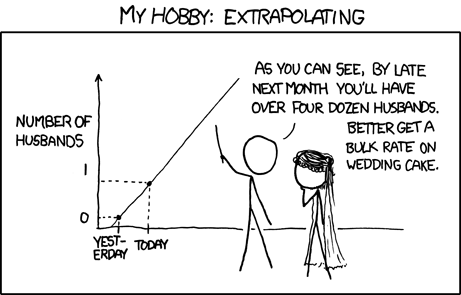
\includegraphics[width=0.6\textwidth]{images/extrapolating.png}

Credit: www.xkcd.com
\end{center}

\end{frame}


\begin{frame}
\Large

\begin{center}
Chi-Squared Test\footnote{Is not a test, and does not involve chi squared.}
\end{center}
\end{frame}


\begin{frame}
\frametitle{Motivating Example}

\begin{center}
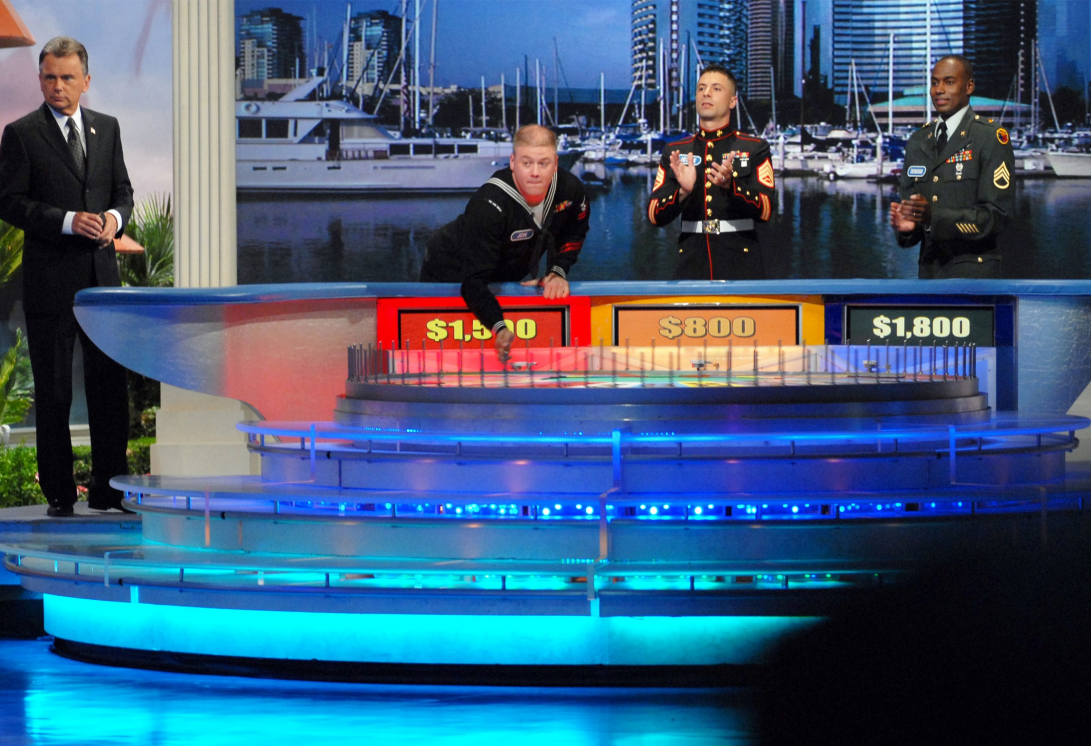
\includegraphics[width=0.6\textwidth]{images/wheel_of_fortune.png}

Source: Wikimedia Commons
\end{center}

\end{frame}


\begin{frame}
\frametitle{The Data}
The outcomes of $N=30$ Wheel of Fortune episodes:

\begin{center}
\begin{tabular}{|c|ccc|}
\hline
Position & 1 & 2 & 3 \\
\hline
Number of Wins $x$ & 8 & 9 & 13 \\
\hline 
\end{tabular}
\end{center}

\end{frame}

\begin{frame}
\frametitle{The Question}
We might wonder whether the following hypothesis is true:\\[0.5em]\pause

$H_0$: There is a 1/3 probability for each position to win each episode.

\end{frame}

\begin{frame}[fragile]
\frametitle{Classical Chi-Squared Test}
The classical `chi-squared test' is designed for this situation.
The test statistic is based on the difference between the observed counts
(8, 9, 13) and the expected counts under $H_0$ (10, 10, 10).
\pause
\begin{minted}{r}
> chisq.test(c(8, 9, 13))

	Chi-squared test for given probabilities

data:  c(8, 9, 13)
X-squared = 1.4, df = 2, p-value = 0.4966
\end{minted}

\end{frame}

\begin{frame}[fragile]
\frametitle{Classical Chi-Squared Test}
The main {\bf advantage} of the classical chi-squared test is that it is very
easy to carry out because it is already implemented in R.\\[0.5em]\pause

The main {\bf disadvantages} are:\pause
\begin{itemize}
\item It returns a p-value, not a posterior probability, and is subject to the
usual objections.\pause
\item It is based on an approximation that assumes that the number of counts
in each bin is high. Typically $\geq 5$ is preferred.
\end{itemize}

\end{frame}


\begin{frame}
\frametitle{Let's Make it Bayesian}
\begin{itemize}
\item Think of it as parameter estimation.\pause
\item There are $N$ trials and we will assume that, on each trial, the
probabilities for each `bin' are $(\theta_1, \theta_2, \theta_3)$.\pause
\item We will get the posterior distribution for the $\theta$ parameters
given the $x$ data (counts).\pause
\item This will involve two new distributions: the {\bf Dirichlet} for the
prior and the {\bf Multinomial} for the sampling distribution.
\end{itemize}

\end{frame}

\begin{frame}
\frametitle{From Binomial to Multinomial}

\begin{itemize}
\item Binomial situation: $N$ trials, success (with probability $\theta$)
or failure $(1-\theta)$ on each trial. We observe $x$ successes and $(N-x)$
failures, and the binomial distribution applies to $x$.\pause
\item Multinomial situation: $N$ trials, with bin probabilities
$\theta_1, \theta_2, ..., \theta_M$. We observe the counts in each bin,
$x_1, ..., x_M$.
\end{itemize}

\end{frame}

\begin{frame}
\frametitle{From Binomial to Multinomial}
The expression for the multinomial distribution is:

\begin{align}
p(x_1, ..., x_m \given \theta_1, ..., \theta_m)
    &= \frac{N!}{x_1!x_2!...x_M!}\theta_1^{x_1}\theta_2^{x_2}...\theta_M^{x_M}.
\end{align}
\pause

This gives the probability of obtaining $x_1$ outcomes in bin 1,
$x_2$ outcomes in bin 2, and so on, when the probabilities
of each bin on each trial are given by the $\theta$ parameters.

\end{frame}


\begin{frame}
\frametitle{Important Constraints}
We have important constraints on the parameters ($\theta$s) and the counts
($x$s):

\begin{align}
\theta_1 + \theta_2 + ... + \theta_M &= 1 \\
x_1 + x_2 + ... + x_M &= N.
\end{align}

\end{frame}


\begin{frame}
\frametitle{From Multinomial to Binomial}
If there are $M=2$ bins, and we call one `success' and the other `failure',
then the multinomial distribution becomes

\begin{align}
p(x_1, x_2 \given \theta_1, \theta_2)
    &= \frac{N!}{x_1!x_2!}\theta_1^{x_1}\theta_2^{x_2}.
\end{align}

which is an alternative way of writing the Binomial distribution

\begin{align}
p(x_1 \given \theta_1)
    &= \binom{N}{x_1}\theta_1^{x_1}(1 - \theta_1)^{N - x_1}.
\end{align}


\end{frame}

\end{document}

